\chapter{Richtcharakteristik (kreisf"ormiger) Lautsprecher \label{chapter:kreis}}
\lhead{Richtcharakteristik (kreisf"ormiger) Lautsprecher}
\begin{refsection}
\chapterauthor{Kevin Cina und Benjamin R"aber}
\\
%
%
%%Text ist für mich noch nicht zufriedenstellend
%In diesem Kapitel geht es um die \emph{Richtcharakteristik von kreisf\"ormigen Antennen}.
%Vorweg genommen bekommt man die \emph{Besselfunktion} als L\"osung.
%Die Herleitung ist aber allgemein f\"ur aller zylindrische K\"orper anwendbar.
%F\"ur das bessere Verst\"andnis wird zuerst der Weg von einer rechteckigen Pauke zu einer kreisf\"ormigen Pauke gemacht und erst danach kommen wir zum Thema \emph{Richtcharakteristik von kreisf\"ormigen Antennen}.
%
%
%
%Potenzreihenherleitung
\section{Potenzreihenherleitung der Besselfunktion}
Das Ziel dieses Abschnittes ist, die Besselfunktion mit der Potenzreihen-Methode die in Kapitel \ref{section:potenzreihen:verallgemeinert} erl\"autert wurde, herzuleiten.
\dots \\
%Dieser Abschnitt befasst sich mit der Potenzherleitung der Besselfunktion. 
%Bei der Herleitung werden Methoden, die in den vorherigen Kapitel  erl\"autert wurden, 
%verwendet. Zuerst m\"uss eine Differenzialgleichung aufgestellt werden.
%Die Besselfunktion kommt aus der Wellengleichung.
%
\dots So kommt man auf die Gleichung \ref{eq:bessel_dgl}, welche grosse \"Ahnlichkeit mit der Gleichung \ref{potenzreihen:verallgemeinert-bessel} aufweisst.
%Die Differenzialgleichung f\"ur die Besselfunktion lautet wiefolgt:
\begin{align}
	r^2 \, R'' \left( r \right)
	+
	r \, R' \left( r \right)
	+
	\left( r^2 - n^2 \right) \, R \left( r \right)
	=
	0
	\label{eq:bessel_dgl}
\end{align}
Im Folgenden wird nun die Gleichung \ref{eq:bessel_dgl}, mithilfe der Potenzreihen-Methode aus dem Kapitel \ref{section:potenzreihen:verallgemeinert}, gel\"ost und der L\"osungsweg aufgezeigt.
\subsection*{Vorgehensweise}
\begin{enumerate}
	\item Die Potenzreihe und deren Ableitungen berechnet.
	\item Die Potenzreihen in die Differenzialgleichung \ref{eq:bessel_dgl} eingesetzen, um
	\item die Indexgleichung f\"ur $\varrho$ zu l\"osen, welche
	\item eine Rekursion der Koeffizienten erm\"oglicht.
	\item Bestimmen der Koeffizienten f\"ur
	\item die Besselfunktion mit ganzzahlige Parametern \ref{eq:bessel_summenformel}.
%	\item Allgemeine Besselfunktion \ref{eq:bessel_summenformel:allgemein}
\end{enumerate}


%Um die Differenzialgleichung zu l\"osen, w\"ahlen wir den Potenzreihenansatz mit der folgenden Potenzreihe und deren Ableitungen:
\subsection*{Potenzreihe und deren Ableitungen}
\begin{align*}
	R \left( r \right)
	&=
	r^{\varrho}
	\sum_{k=0}^{\infty} a_k \, r^k
\\
	R'\left( r \right)
	&=
	\varrho \, r^{\varrho - 1}
	\sum_{k=0}^{\infty} a_k \, r^k
	+
	r^{\varrho}
	\sum_{k=0}^{\infty} a_k \, k \, r^{k - 1}
\\
	R'' \left( r \right)
	&=
	\varrho \, \left( \varrho - 1 \right) \, r^{\varrho - 2}
	\sum_{k=0}^{\infty} a_k \, r^k
	+
	2 \, \varrho \, r^{\varrho - 1}
	\sum_{k=0}^{\infty} a_k \, k \, r^{k - 1}
	+
	r^{\varrho}
	\sum_{k=0}^{\infty} a_k \, k \, \left( k - 1 \right) \, r^{k - 2}	
\end{align*}
\subsection*{Potenzreihen in Differenzialgleichung \ref{eq:bessel_dgl} einsetzen}
%Nun kann man die Potenzreihen in die Differenzialgleichung \ref{eq:bessel_dgl} einsetzen und bekommt dann:
\begin{align*}
	\overbrace{
		\varrho \, \left( \varrho - 1 \right) \, r^{\varrho}
		\sum_{k=0}^{\infty} a_k \, r^k
		+
		2 \, \varrho \, r^{\varrho}
		\sum_{k=0}^{\infty} a_k \, k \, r^k
		+
		r^{\varrho}
		\sum_{k=0}^{\infty} a_k \, k \, \left( k - 1 \right) \, r^k
	}^{r^2 \, R''\left( r \right)}
	+ \\
	\overbrace{
		\varrho \, r^{\varrho}
		\sum_{k=0}^{\infty} a_k \, r^k
		+
		r^{\varrho}
		\sum_{k=0}^{\infty} a_k \, k \, r^k
	}^{r \, R' \left( r \right)}
	+\\
	\overbrace{
	r^{\varrho}
		\sum_{k=0}^{\infty} a_k \, r^{\textcolor{red}{k + 2}}
		-
		n^2 \, r^{\varrho}
		\sum_{k=0}^{\infty} a_k \, r^k
	}^{\left( r^2 - n^2 \right) \, R \left( r \right)}
	= & \, 0
\end{align*}
%Gleiche Summenzeichen zusammenfassen:
\begin{align*}
	\left(
	\varrho \, \left( \varrho - 1 \right)
	+
	\varrho
	-
	n^2
	\right)
	\, r^{\varrho}
	\sum_{k=0}^{\infty} a_k \, r^k
	+ \\
	\left(	
	2 \, \varrho
	+
	1
	\right)
	\, r^{\varrho}
	\sum_{k=0}^{\infty} a_k \, k \, r^k
	+ \\
	r^{\varrho}
	\sum_{k=0}^{\infty} a_k \, k \, \left( k - 1 \right) \, r^k
	+ \\
	r^{\varrho}
	\sum_{k=0}^{\infty} a_k \, r^{\textcolor{red}{k + 2}}
	= & \, 0
\end{align*}
\subsection*{Indexgleichung f\"ur $\varrho$}
%Nun muss man eine Indexgleichung für die Unbekannte $\varrho$ aufstellen, um diese zu bestimmen.
%\ref{section:potenzreihen:verallgemeinert}
%Dazu eignet sich eine Indexgleichung f\"ur den Koeffizienten $a_0$:
\begin{align*}
%	\left( \varrho \, \left( \varrho -1 \right) + \varrho - n^2 \right) \, a_0 &= 0 && \left| :a_0 \right. \\
	\varrho \, \left( \varrho -1 \right) + \varrho - n^2 &= 0 && \left| \text{Ausmultiplizieren} \right. \\
	\varrho ^2 - \varrho + \varrho -n^2 &= 0 && \left| \text{Vereinfachen} \right.\\
	\varrho ^2 - n^2 &= 0 && \left| +n^2 \right.\\
	\varrho ^2 &= n^2 && \left| \sqrt{\centerdot} \right. \\
	\varrho &= \pm n \text{ und } \\
	\varrho &= \pm 0 %\left( \text{Doppelte Nullstelle} \right)
\end{align*}
%Wir beschr\"anken uns in diesem Kapitel nur mit der L\"oesung $\varrho = \pm n$. Die L\"osung f\"ur $\varrho = \pm 0$ wird im Kapitel \ref{chapter:komplex} genauer behandelt.
%Nun kann man $n$ f\"ur $\varrho$ in die Gleichung einsetzen und erh\"alt:
\begin{align*}
	\left(
	n \, \left( n - 1 \right)
	+
	n
	-
	n^2
	\right)
	\, r^{n}
	\sum_{k=0}^{\infty} a_k \, r^k
	+ \\
	\left(	
	2 \, n
	+
	1
	\right)
	\, r^{n}
	\sum_{k=0}^{\infty} a_k \, k \, r^k
	+ \\
	r^{n}
	\sum_{k=0}^{\infty} a_k \, k \, \left( k - 1 \right) \, r^k
	+ \\
	r^{n}
	\sum_{k=0}^{\infty} a_k \, r^{\textcolor{red}{k + 2}}
	= & \, 0
\end{align*}
%Als n\"achstes fasst man alles in eine einzige Summe zusammen und vereinfacht diese:
\begin{align*}
	r^n
	\sum_{\textcolor{red}{k=2}}^{\infty}
	\left( n \, \left( n - 1 \right) \, a_k
	+
	2 \, n \, k \, a_k
	+
	k \, \left( k - 1 \right) \, a_k
	+
	n \, a_k
	+
	k \, a_k
	+
	a_{k-2}
	-
	n^2 \, a_k
	\right)
	\, r^k
	= 0 \\
	%
	r^n
	\sum_{k=2}^{\infty}
	\left(
	2 \, n \, k \, a_k
	+
	k^2 \, a_k
	+
	a_{k - 2}
	\right)
	\, r^k
	= 0
\end{align*}
%Weil $r \neq 0$ sein muss, muss $ \left( 2 \, n \, k + k^2 \right) \, a_k + a_{k - 2} = 0$ sein.
%Nun kann man eine Rekursion der Koeffizienten $a_k$ berechnen.
\begin{align}
	a_k
	=
	\frac
	{
		-a_{k - 2}
	}{
		k \, \left( 2 \, n + k \right)	
	}
	\label{eq:bessel_koeffreq}
\end{align}
%Da $k \geq 0$ sein muss, sind nur gerade Koeffizienten m\"oglich. Somit kann man f\"ur $k$ nun $2k$ in die Gleichung \ref{eq:bessel_koeffreq} einsetzen und erh\"alt:
\begin{align*}
	a_{2k}
	&=
	\frac
	{
		-a_{2k - 2}
	}{
		2k \, \left( 2 \, n + 2k \right)	
	} \\
	&=
	\frac
	{
		-a_{2k - 2}
	}{
		4k \, \left( n + k \right)	
	} \\
	&=
	\frac
	{
		-a_0
	}{
		4^k \, {k}! \, {\left( n + k \right)}!
	} \\
	&=
	\frac
	{
		-a_0
	}{
		2^{2k} \, {k}! \, {\left( n + k \right)}!
	}
\end{align*}
%Setzt man nun f\"ur $a_0 = \frac{1}{2^n \, {n}!}$ ein, so kommt man auf die Form:
\begin{align}
	J_n \left( r \right)
	&= \nonumber
	\sum_{k=0} ^{\infty}
	\frac
	{
		\left( - 1 \right) ^k \, r ^{2k+n}
	}{
		2^{2k+n} \, {k}! \, { \left( k + n \right) }!
	} \\
	&= \nonumber
	\sum_{k=0} ^{\infty}
	\frac
	{
		\left( - 1 \right) ^k \, 
		\frac
		{
			r ^{2k+n}
		}{
			2^{2k+n}
		}
	}{
		{k}! \, { \left( k + n \right) }!
	} \\
	&=
	\sum_{k=0} ^{\infty}
	\frac
	{
		\left( - 1 \right) ^k \, 
		\left(		
		\frac
		{
			r
		}{
			2
		} \right) ^{2k+n}
	}{
		{k}! \, { \left( k + n \right) }!
	}
	\label{eq:bessel_summenformel}
\end{align}
%%	Die Gleichung ist für ganzzahlige Koeffizienten.
%%	Übergang zu Gammafunktion erläutern für allgemeine Formel
%$\Gamma \left( \alpha \right) = {\left( \alpha - 1 \right) }!$
%\begin{align}
%	J_{\pm n} \left( r \right)
%	&=
%	\sum_{k=0} ^{\infty}
%	\frac
%	{
%		\left( - 1 \right) ^k \, 
%		\left(		
%		\frac
%		{
%			r
%		}{
%			2
%		} \right) ^{2k+n}
%	}{
%		{k}! \, \Gamma \left( k + n + 1 \right)
%	}
%	\label{eq:bessel_summenformel:allgemein}
%\end{align}


\begin{figure}
	\begin{center}
		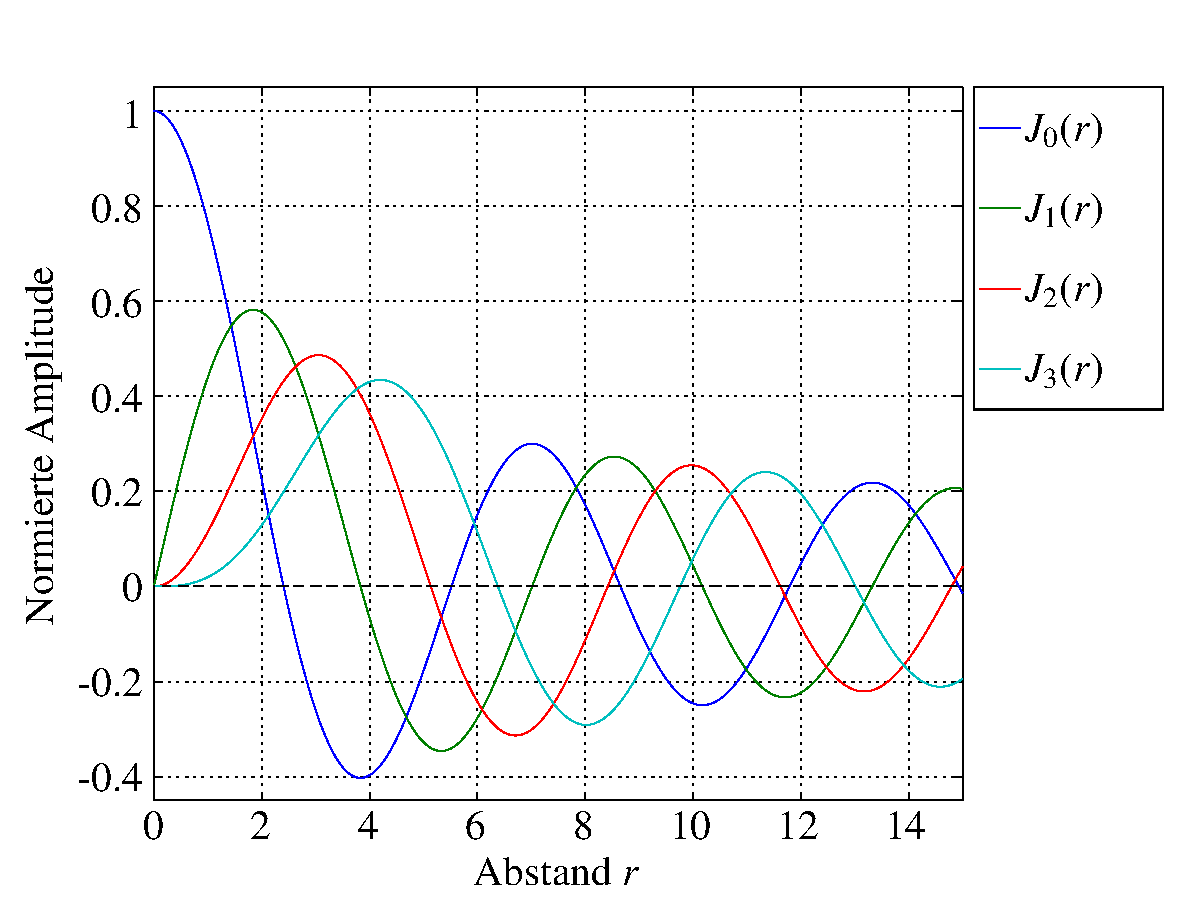
\includegraphics[scale=0.5]{kreis/besselfunction.pdf}
		\label{img:besselfunction}
		\caption[Besselfunktion]{Besselfunktion geplottet}
	\end{center}
\end{figure}

\newpage

\subsection{Veranschaulichung der Besselfunktion mit Beispielen}

\printbibliography[heading=subbibliography]
\end{refsection}

